% Frozen all-32 checkpoint measurements.
\begin{table}[!htb]\centering\footnotesize\setlength{\tabcolsep}{3pt}
\caption{Gauge-solver accuracy and cost at the fixed checkpoint. \docref{Figure}{fig:gauge-solver-ablation} plots the Poisson residual $\epsilon_P$. Harmonic overlap and tangential trace are percentages; all four timing columns are seconds. Size denotes grid size or retained spline degrees of freedom. Setup and assessment are excluded from forward/reverse. Superscript R denotes a synchronized measurement of the complete workload; forward/reverse columns exclude setup and assessment.}
\label{tab:gauge-solver-ablation}

\begin{tabular}{lrrrrrrr}\toprule
Method&Size&Harm.&Wall tan.&Forward&Reverse&Setup&Assess.\\\midrule
Fourier--MFS & $193^3$ & 0.0177 & 0.6904 & 49.07 & 138.60 & $54.57^{\mathrm R}$ & $23.82^{\mathrm R}$\\
Fourier--MFS, reuse & $193^3$ & 0.0177 & 0.6904 & 48.28 & 136.12 & $62.86^{\mathrm R}$ & $23.32^{\mathrm R}$\\
Spline 12 & 3,106 & 0.0181 & 0.0012 & 6.63 & 6.98 & 1.98 & 5.90\\
Spline 20 & 10,648 & 0.0015 & 0.0012 & 15.40 & 16.60 & 4.75 & 5.91\\
Spline 24 + two-level & 17,086 & 0.0036 & 0.0012 & 71.00 & 78.96 & 11.69 & 5.84\\
Volume FMM 32 & $32^3$ & 0.0242 & 4.8727 & 12.15 & 13.43 & 22.99 & 61.76\\
Volume FMM 64 & $64^3$ & 0.0261 & 3.6399 & 14.23 & 17.66 & 22.82 & 60.63\\
Volume FMM 64 adaptive & $64^3$ & 0.0261 & 3.6399 & 14.53 & 17.96 & 23.71 & 60.51\\\bottomrule\end{tabular}\end{table}

Forward and reverse totals include synchronized component measurements; one-time setup and independent assessment are separate columns. Setup combines spline space/quadrature and optional multigrid construction, or the FMM and fixed harmonic moments; assessment combines independent residual, harmonic, and wall checks. Spline forward timing includes query-point construction. The Fourier and Fourier-reuse measurements share identical neural passes and include source-array export, while spline and volume methods use in-memory sources. Both particular-solution families reuse the geometry-dependent MFS factors.

\begin{table}[!htb]
\centering\small
\caption{Floating-point precision on the same $193^3$ grid. The first two rows use identical source samples. Source time measures one all-32 forward pass, including export.}
\label{tab:gauge-precision}
\begin{tabular}{lrr}\toprule
Arithmetic & $\epsilon_P$ (\%) & Source forward (s)\\\midrule
Training arithmetic & 7.989593 & 37.24 \\
FP32 source, FP64 FFT & 7.989595 & 37.24 \\
FP64 source and FFT & 7.989582 & 266.41 \\
\bottomrule\end{tabular}\end{table}
\paragraph{Representation and arithmetic.}
The precision controls yield nearly identical forcing residuals (\docref{Table}{tab:gauge-precision}). With identical source samples, changing FFT precision produces a relative Laplacian difference of $4.20\times10^{-7}$. Source-space resolution therefore provides the effective control over representative selection at this checkpoint.

Transform reuse preserves forward outputs to the reported precision and changes the source cotangent by a relative $2.50\times10^{-12}$. It reduces the three-evaluation Fourier stage from 9.91 to 8.99 seconds and the source-grid transpose from 12.96 to 10.48 seconds. Total component time decreases from 187.67 to 184.40 seconds (1.74\%); neural source evaluation and parameter differentiation account for 85.5\% of the original total.

\paragraph{Auxiliary-space resolution.}
Refinement systematically improves the spline and volume corrections (\docref{Figure}{fig:gauge-solver-ablation}), while the harmonic projection maintains small overlap across the solver family (\docref{Table}{tab:gauge-solver-ablation}). These complementary diagnostics identify two controls for representative selection: the approximation space resolves gradient content, and the mass projection selects harmonic coordinates. Source adaptation refines 31,432 of 32,768 coarse cells (95.9\%), with 284,224 source evaluations including the coarse pass, compared with 262,144 for the uniform rule. This distribution favors uniform refinement for the present forcing.
\paragraph{Operator consistency.}
FMM evaluation and transpose consistency are tested using $16^3$ cuboids, 48 query points, and two random right-hand sides. The analytic cuboid kernel agrees with nonsingular Gauss integration to relative $7.30\times10^{-11}$. Against direct cuboid integration, increasing the far expansion degree from four to six reduces relative gradient error from $1.38\times10^{-3}$ to $1.90\times10^{-4}$; the degree-six transpose discrepancy is $2.73\times10^{-16}$. These comparisons isolate evaluation of the chosen density from density approximation. For the manufactured scalar $e(x)[1+0.2\sin(2\pi x_1)+0.1x_2x_3]$, the refined spline method gives relative gradient and Poisson errors of $2.85\times10^{-4}$ and $8.82\times10^{-4}$, with linear residual $4.95\times10^{-9}$. Together with \docref{Figure}{fig:gauge-solver-ablation} and \docref{Table}{tab:gauge-solver-ablation}, these checks connect accurate operator evaluation to systematic control through auxiliary-space refinement.

\begin{figure}[!htb]
\centering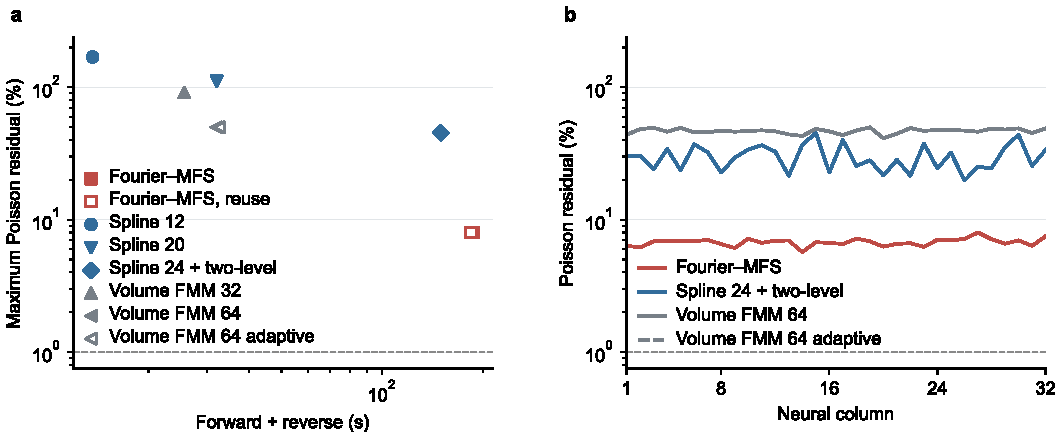
\includegraphics[width=\linewidth,height=.72\textheight,keepaspectratio]{gauge_solver_ablation.pdf}
\caption{\textbf{Gauge-solver accuracy and cost.} Left: all-32 forward-plus-reverse time versus independent Poisson residual. Right: per-column residuals for Fourier--MFS and the finest tested spline and volume spaces. All methods evaluate the same fixed neural checkpoint.}
\label{fig:gauge-solver-ablation}
\end{figure}
